\documentclass{article}
\usepackage{graphicx, fancyhdr, amsmath}
\usepackage[margin=0.6in, top=1in]{geometry}
\usepackage{float}
\usepackage[absolute, overlay]{textpos}
\usepackage[colorlinks=true, linkcolor=blue]{hyperref}

\pagestyle{fancy}
\fancyhf{}
\renewcommand{\headrulewidth}{0pt}

\fancyhead[L]{
\begin{textblock*}{2cm}(0.3in,0.1in)  % {block width} (x-coordinate, y-coordinate)
    
\includegraphics[width=2cm]{NEW LOGO.png}  % Example image placeholder
\end{textblock*}
}
\fancyhead[R]{Math Success Program, UCLA}
\fancyfoot[R]{Created for the MSP by Asmi Kawatkar}

\fancypagestyle{plain}{
}


\title{Review Sheet: Logarithmic \& Exponential Functions}
\date{}
\author{}

\begin{document}
\maketitle
\vspace{-0.75in}
\section*{Content Review}
\subsection*{Overview}

\noindent \textit{Introduction to Exponential \& Logarithmic Functions}
\newline

$e \approx 2.718$ is a number, just like $\pi$. It is most intuitive to think about $e^x$ in comparison to another function like $2^x$ since you are used to thinking about 2 as a number. 
\noindent \newline \textbf{Common mistake}: $e$ is NOT a variable, don't treat it like one.

\noindent
We know that 
\begin{eqnarray*}
    2^x = 1 &\implies& x = 0 \\
    2^x = 2 &\implies& x = 1 \\
    2^x = 4 &\implies& x = 2 \\
    2^x = 10 &\implies& x = ?
\end{eqnarray*}

\noindent To solve the last one, we need to reverse the 'exponentiation' process, using a function called a \textbf{logarithm}. This does the opposite of $2^x$, and essentially divides $x$ by the 'base' (here 2) multiple times and keeps track of how many times it divides. 

\noindent Logarithms are written as the following:
$$\log_2(10) = x$$
And are read as 'log base 2 of 10 is equal to x'. 

\noindent For example: $$\log_2(8) = 3 \implies 2^3 = 8$$

\noindent Similarly for $e^x$: 
\begin{eqnarray*}
    e^x = 1 &\implies& x = 0 \\
    e^x = e &\implies& x = 1\\
    e^x = e^2 &\implies& x = 2 \\
    e^x = 10 &\implies& x = ?
\end{eqnarray*}

\noindent Now we know that to solve the last one, we use $\log_e(10) = x$.

Revisiting the examples above:
\begin{eqnarray*}
    e^x = 1 &\implies& x = \ln(1) = 0\\
    e^x = e &\implies& x = \ln(e) = 1\\
    e^x = e^2 &\implies& x = \ln(e^2) = 2\\
    e^x = 10 &\implies& x = \ln(10)
\end{eqnarray*}

In math, this function $\log_e$ is used so often, that it has a special name: 'natural logarithm' or $\ln(x)$.
\newline

\noindent \textit{Logarithmic Function Rules}

Similar to how you have learned rules for exponents, there exist the following rules for logarithmic functions which are used to significantly simplify logarithmic expressions.

\begin{eqnarray*}
    \ln(a) + \ln(b) &=& \ln(a\cdot b) \\
    \ln(a) - \ln(b) &=& \ln(a-b) \\
    a\ln(b) &=& \ln(b^a) \\
\end{eqnarray*}
. 

\noindent \textit{Calculus of Exponential \& Logarithmic Functions}
\newline

We will take the following as a rule since it's origins are beyond the scope of MATH 31A/B:
$$\frac{d}{dx}2^x = \ln(2)\cdot 2^x$$

\noindent More generally, 
$$\frac{d}{dx}a^x = \ln(a)\cdot a^x \text{ for some real constant } a$$

Following this rule, we see that
$$\frac{d}{dx}e^x = \ln(e)\cdot e^x = 1 \cdot e^x \text{ because we know that } \ln(e) = 1$$

The following can similarly be taken as rules. The last 2 formulae originate from applications of chain rule. 
\begin{eqnarray*}
    \int e^x dx &=& e^x + c \\
    \frac{d}{dx} \ln(x) &=& \frac{1}{x}  \implies \int{\frac{1}{x}} dx = \ln x\\
    \frac{d}{dx} \ln(f(x)) &=& \frac{f'(x)}{f(x)} \\
    \frac{d}{dx} e^{f(x)} &=& f'(x)\cdot e^{f(x)}
\end{eqnarray*}

\textbf{Important Note:} Logarithms will only accept positive values. There can never be an expression like $\ln(0)$ because no constant raised to a power can equal 0 except 0 itself. So $\ln 0$ is undefined. 

\subsection*{Resources}


\noindent\textit{Logarithmic \& Exponential Functions}
\begin{itemize}
    \item \href{https://youtu.be/I9mVUo-bhM8}{Video: Introduction to Related Rates (Organic Chemistry Tutor, 10 min) - with worked examples} 
    \item \href{https://math.colorado.edu/math1300/resources/Exercises_LogarithmicFunction.pdf}{Worksheet: Logarithmic Function (with Solutions)}
    \item \href{http://www.standrewspaisley.com/uploads/6/0/2/3/60230905/exp_and_logs_full_booklet.pdf}{Explainer: Exponentials \& Logarithms (with Worked Examples)}
    \item \href{https://youtu.be/oqHJ5xQYTEI}{Video: Logarithms \& Exponentials Review (Organic Chemistry Tutor, 1h20min) - detailed concept breakdown \& Explanations}
    \item \href{https://youtu.be/zmnh448y_ZU}{Video: Derivatives of Exponentials \& Logarithms (Organic Chemistry Tutor, 42min)}
    \item \href{https://youtu.be/LRbi_pMX1DM}{Video:Logarithms Explained Rules \& Properties, Graphing etc (Organic Chemistry Tutor, 1h23min)}
\end{itemize}


\subsection*{Acknowlegement}
Questions in the Worked Problems section of this sheet have been taken from external sources that have been linked where appropriate. All solutions have been created independently.

\pagebreak
\section*{Worked Problems}
\label{WorkedProblems}
\subsection*{Equations in Logarithms and Exponentials}
Find all solutions to the following equations. If there is no solution, explain clearly why.
\newline \noindent \href{https://tutorial.math.lamar.edu/problems/calci/explogeqns.aspx}{Source}
\begin{enumerate}
    \item $12 - 4e^{7+3x} = 7$
    \begin{figure}[H]
        \centering
        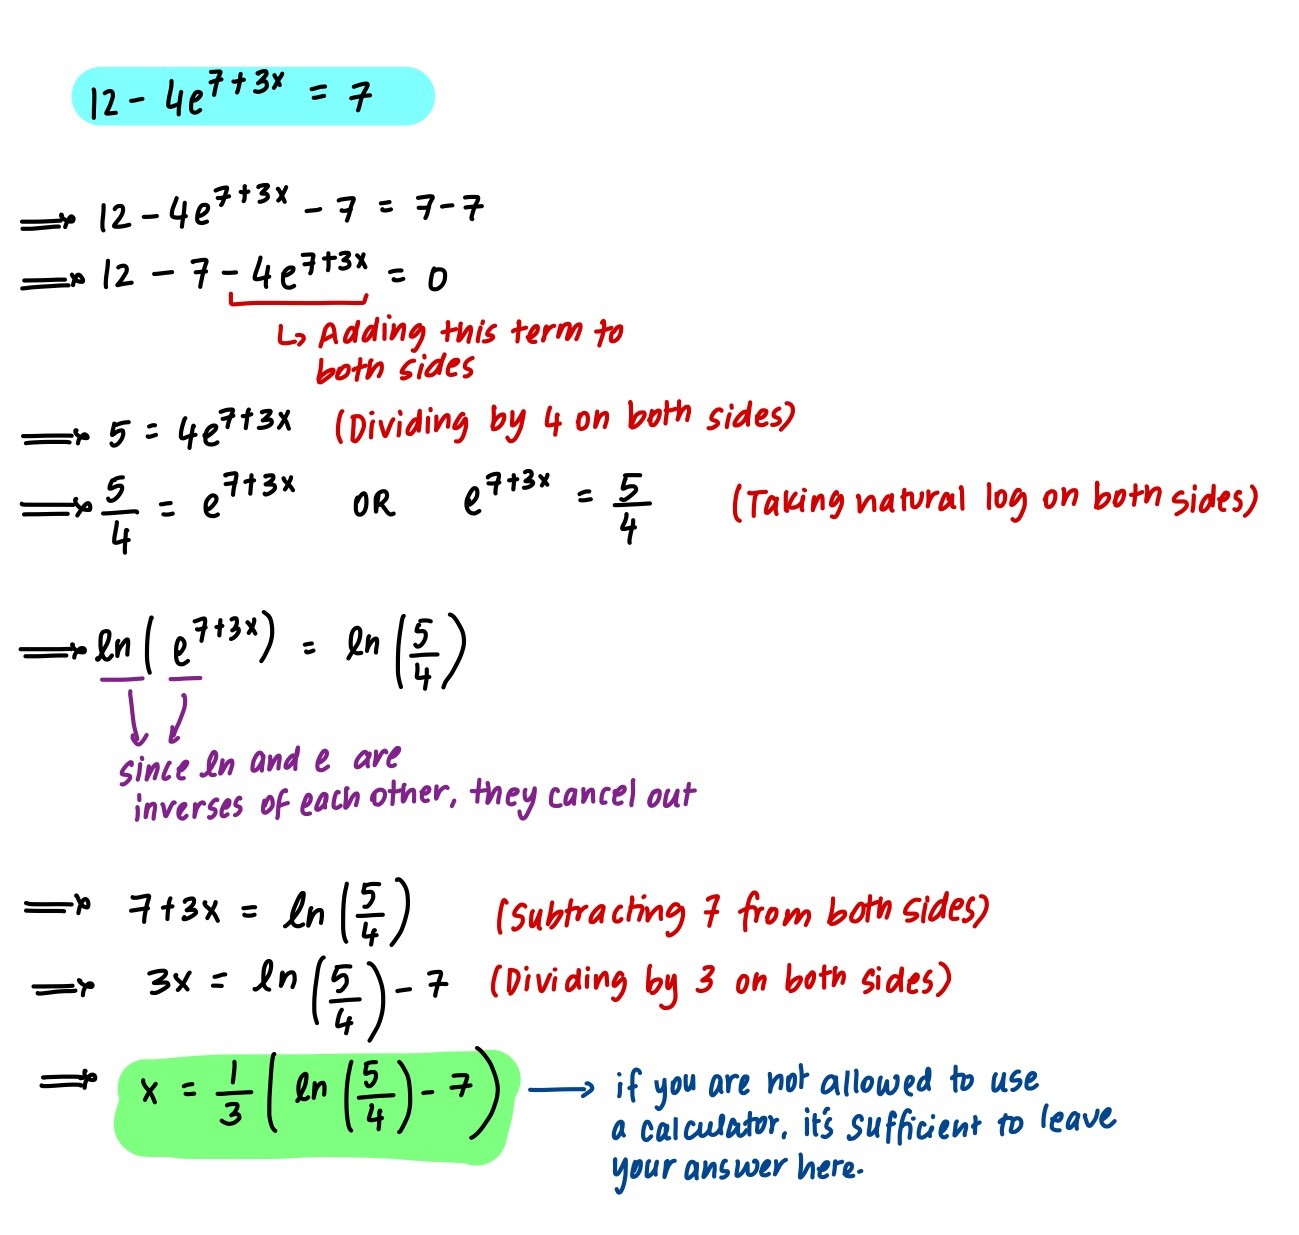
\includegraphics[width=\linewidth]{Q1.jpg}
        \label{fig:Q1}
    \end{figure}
    \newpage
    \item $2t - te^{6t-1} = 0$
    \begin{figure}[H]
        \centering
        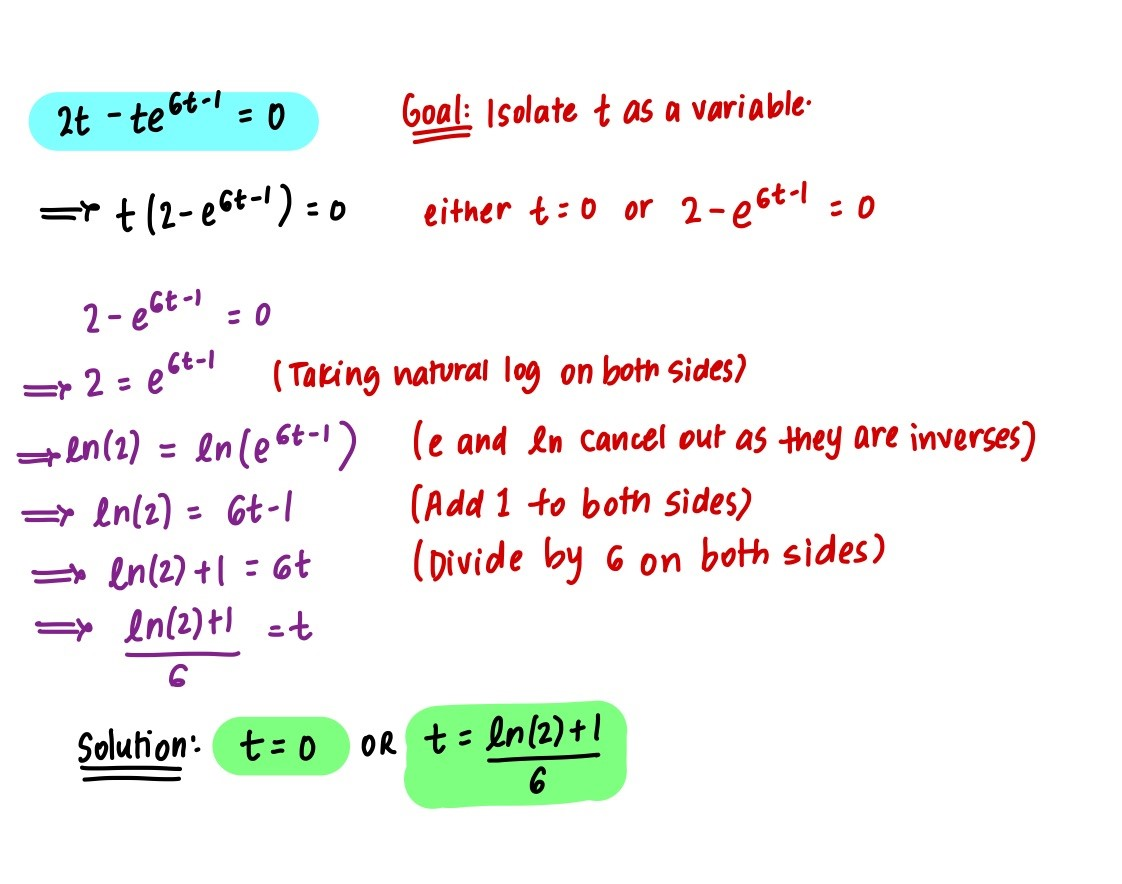
\includegraphics[width=0.75\linewidth]{Q2.jpg}
        \label{fig:Q2}
    \end{figure}
    \item $2\log(x)-\log(7x-1) = 0$
    \begin{figure}[H]
        \centering
        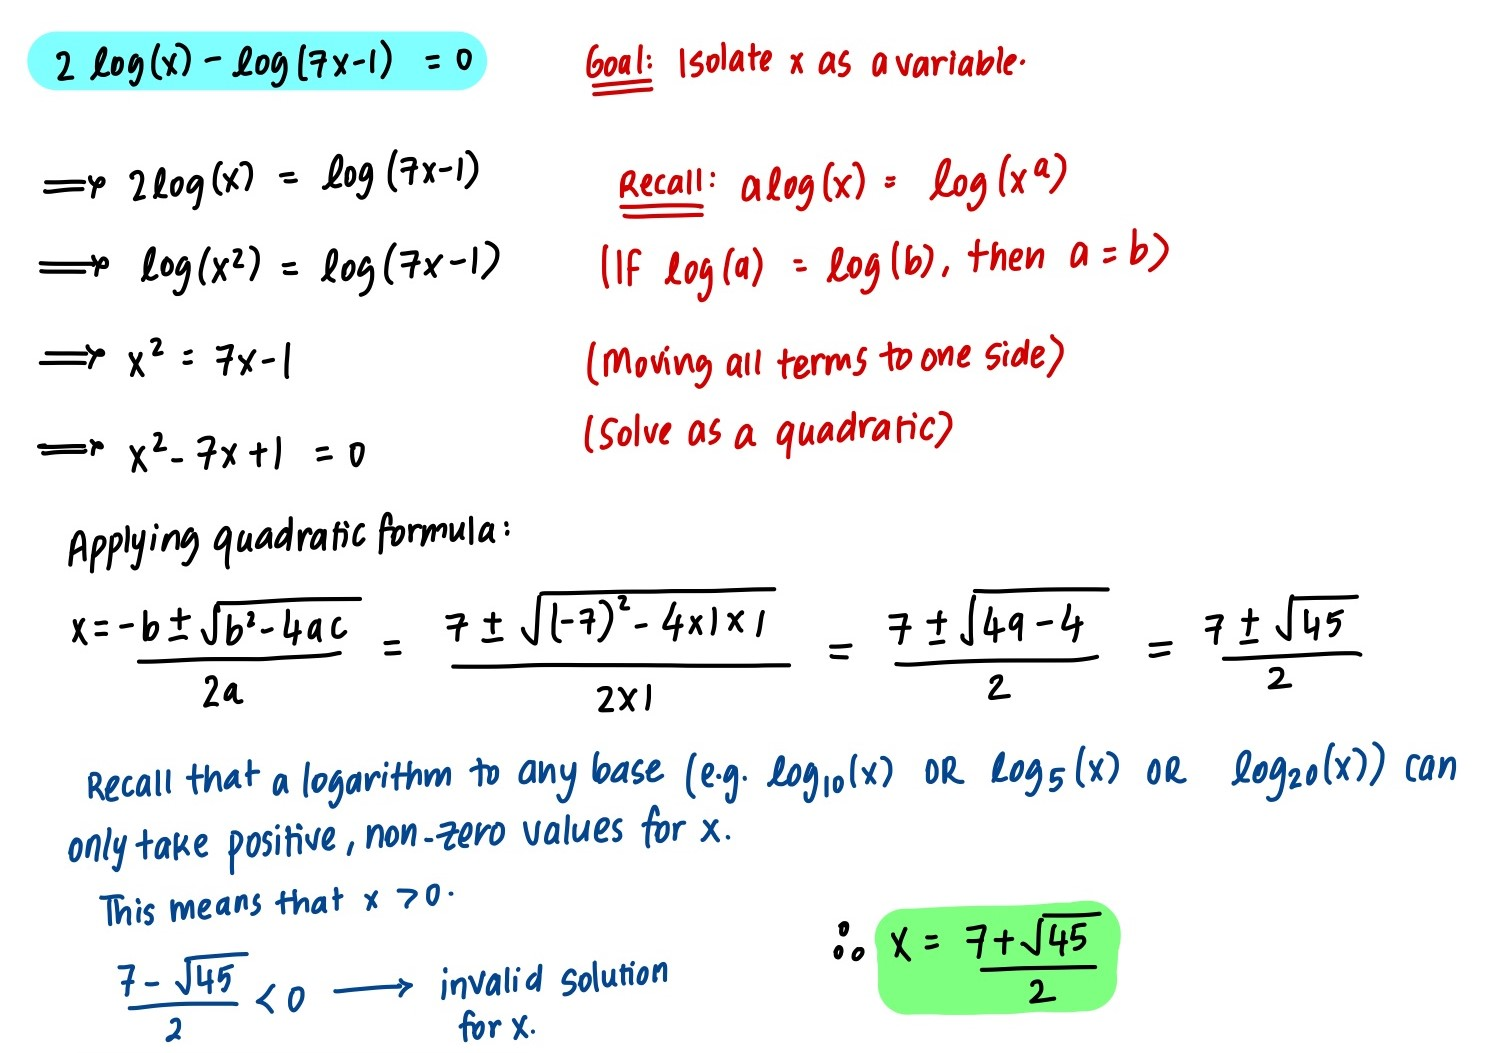
\includegraphics[width=0.8\linewidth]{Q3.jpg}
        \label{fig:Q3}
    \end{figure}
    \item $\ln(y-1)=1+\ln(3y+2)$
    \begin{figure}[H]
        \centering
        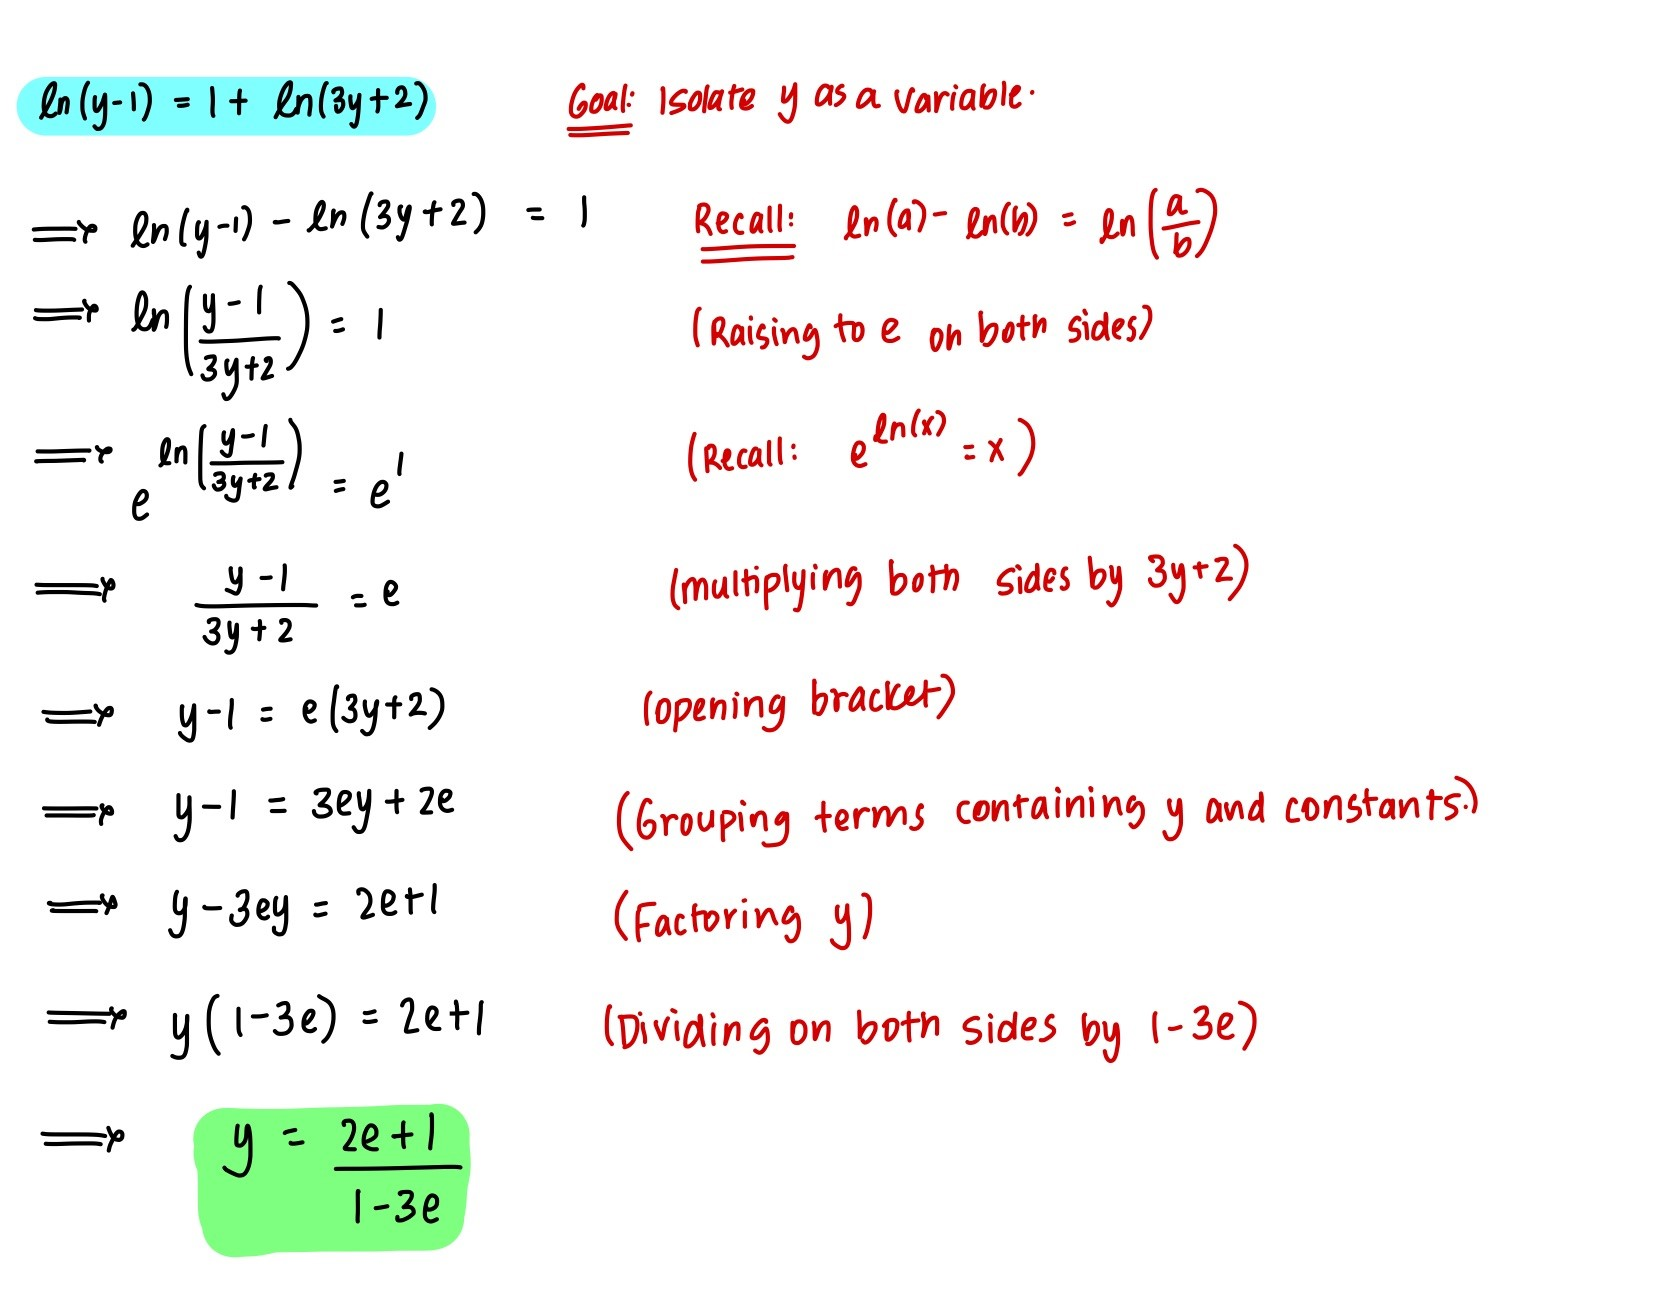
\includegraphics[width=0.9\linewidth]{Q4.jpg}
        \label{fig:Q4}
    \end{figure}
\end{enumerate}

\newpage
\subsection*{Derivatives of Logarithms and Exponentials}
Differentiate the given function.
\noindent \newline \href{https://tutorial.math.lamar.edu/problems/calci/diffexplogfcns.aspx}{Source}

\begin{enumerate}
    \item $f(x) = 2e^x - 8^x$
    \begin{figure}[H]
        \centering
        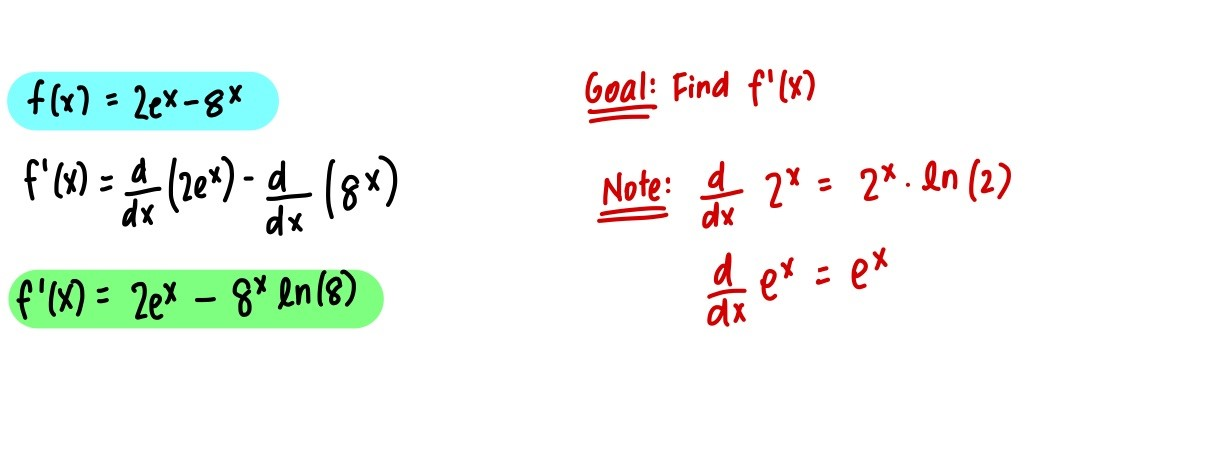
\includegraphics[width=\linewidth]{Q1.1.jpg}
        \label{fig:Q1.1}
    \end{figure}
    \item $y = \ln(x^2 + 1)$
    \begin{figure}[H]
        \centering
        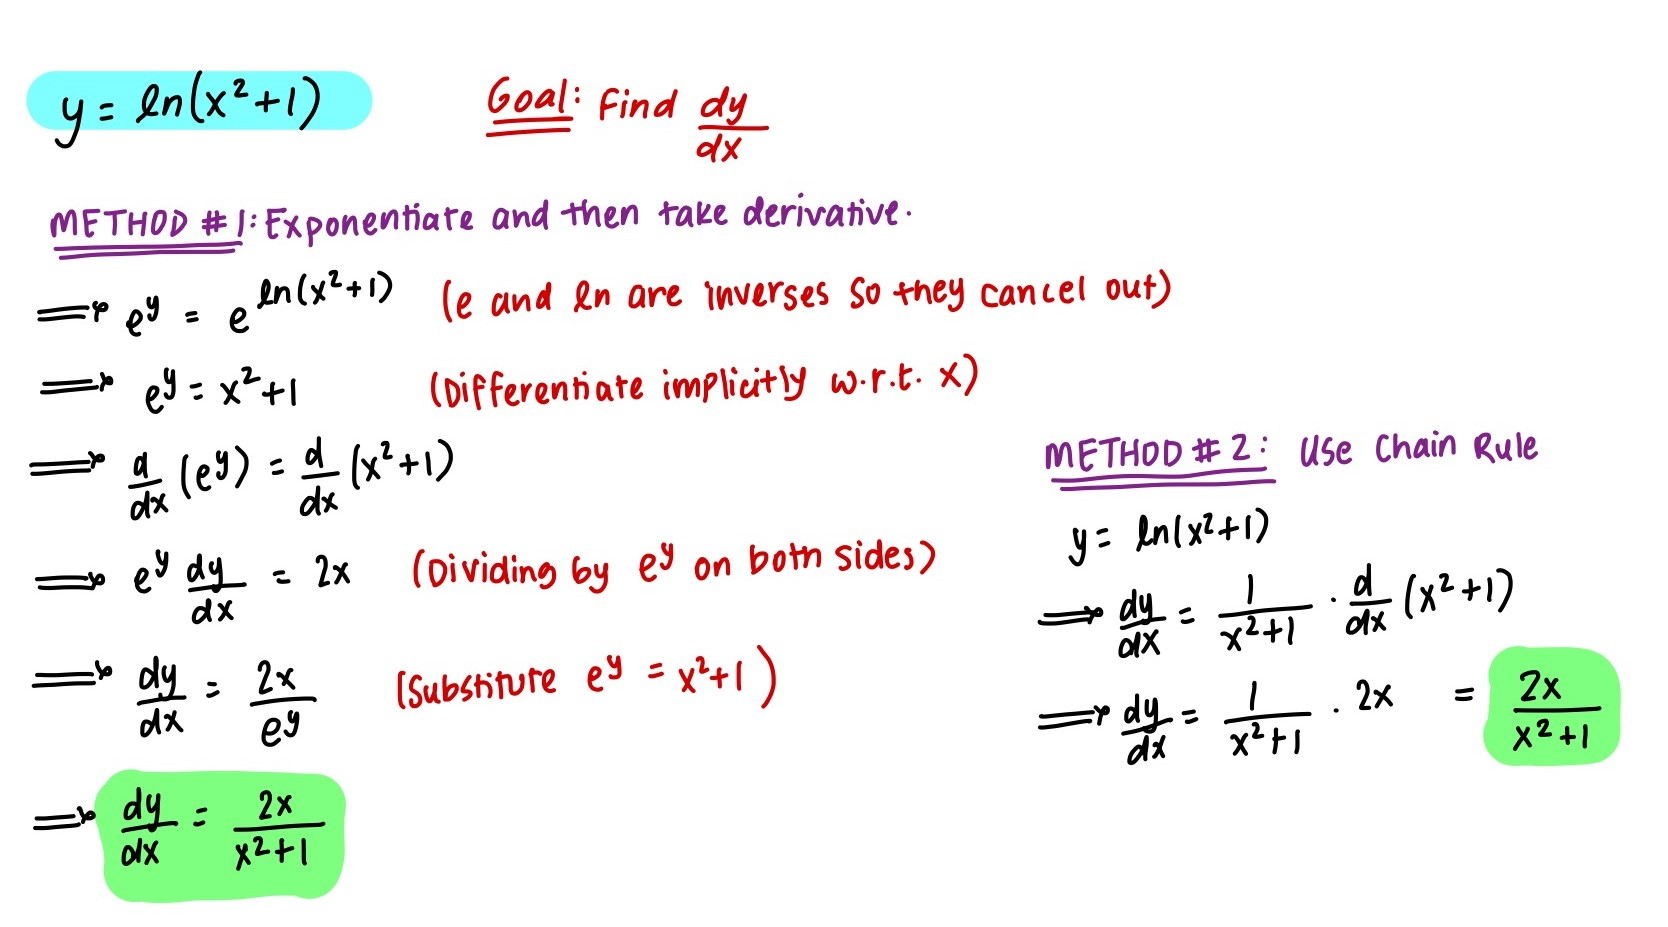
\includegraphics[width=\linewidth]{Q1.6.jpg}
        \label{fig:Q1.6}
    \end{figure}
    \newpage
    \item $y = x^5 -e^x \ln x$
    \begin{figure}[H]
        \centering
        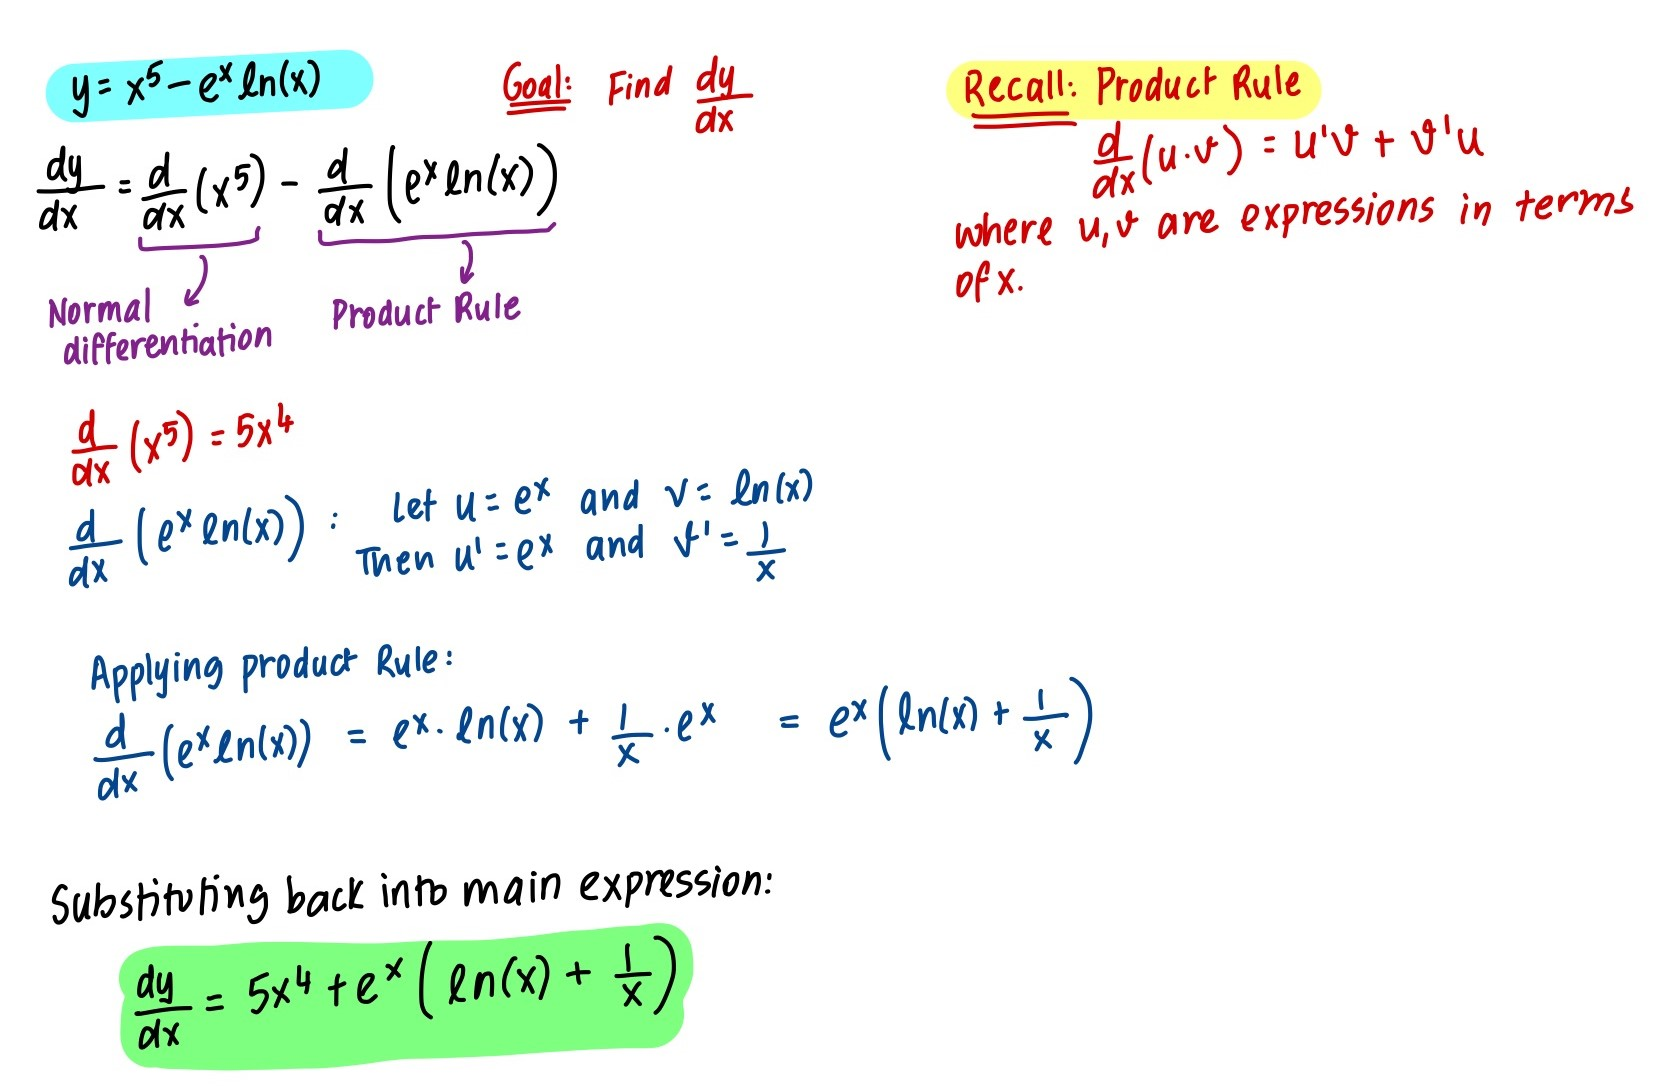
\includegraphics[width=0.9\linewidth]{Q1.2.jpg}
        \label{fig:Q1.2}
    \end{figure}
    \item $y = e^{\ln(x)} + \ln(e^x)$
    \begin{figure}[H]
        \centering
        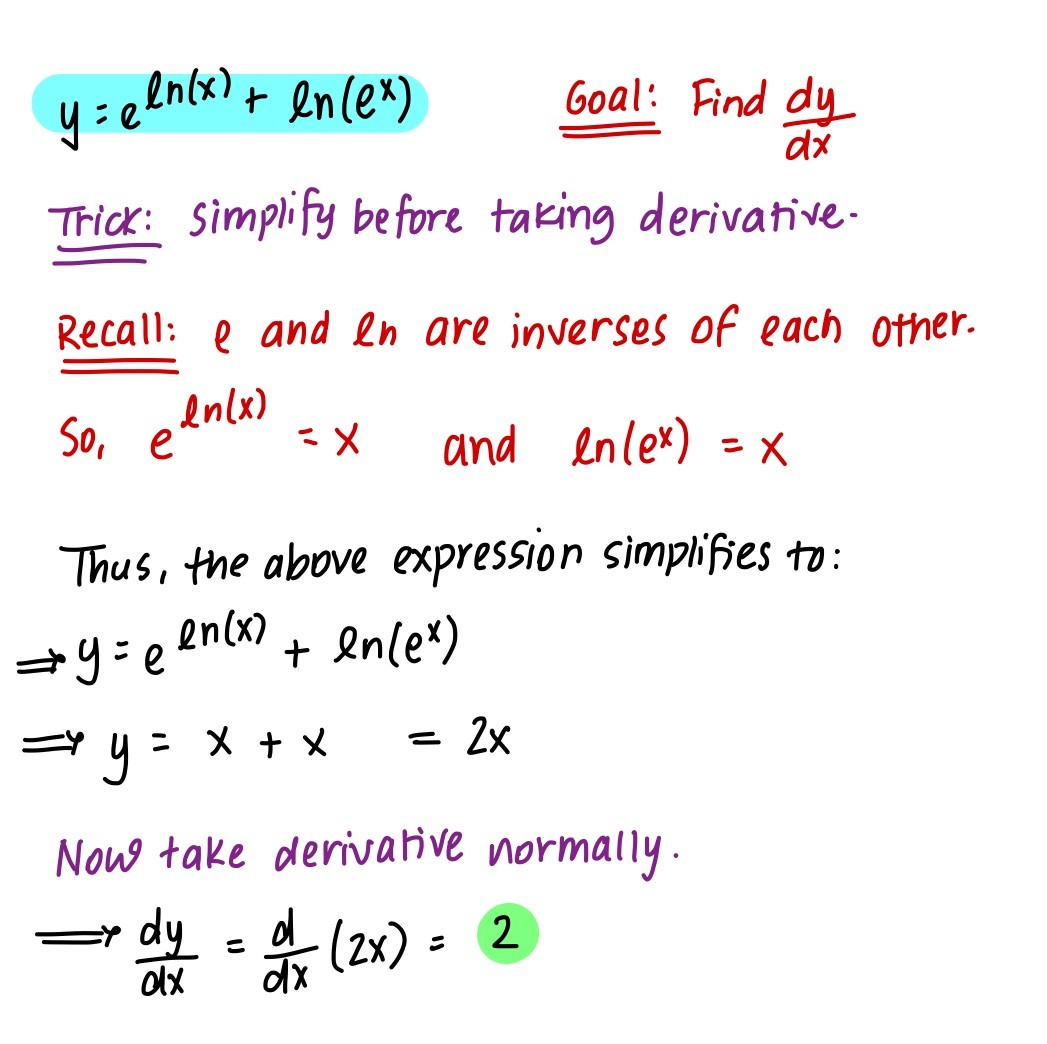
\includegraphics[width=0.55\linewidth]{Q1.5.jpg}
        \label{fig:Q1.5}
    \end{figure}
    \item $y = (x^2 + 1)^x$
    \begin{figure}[H]
        \centering
        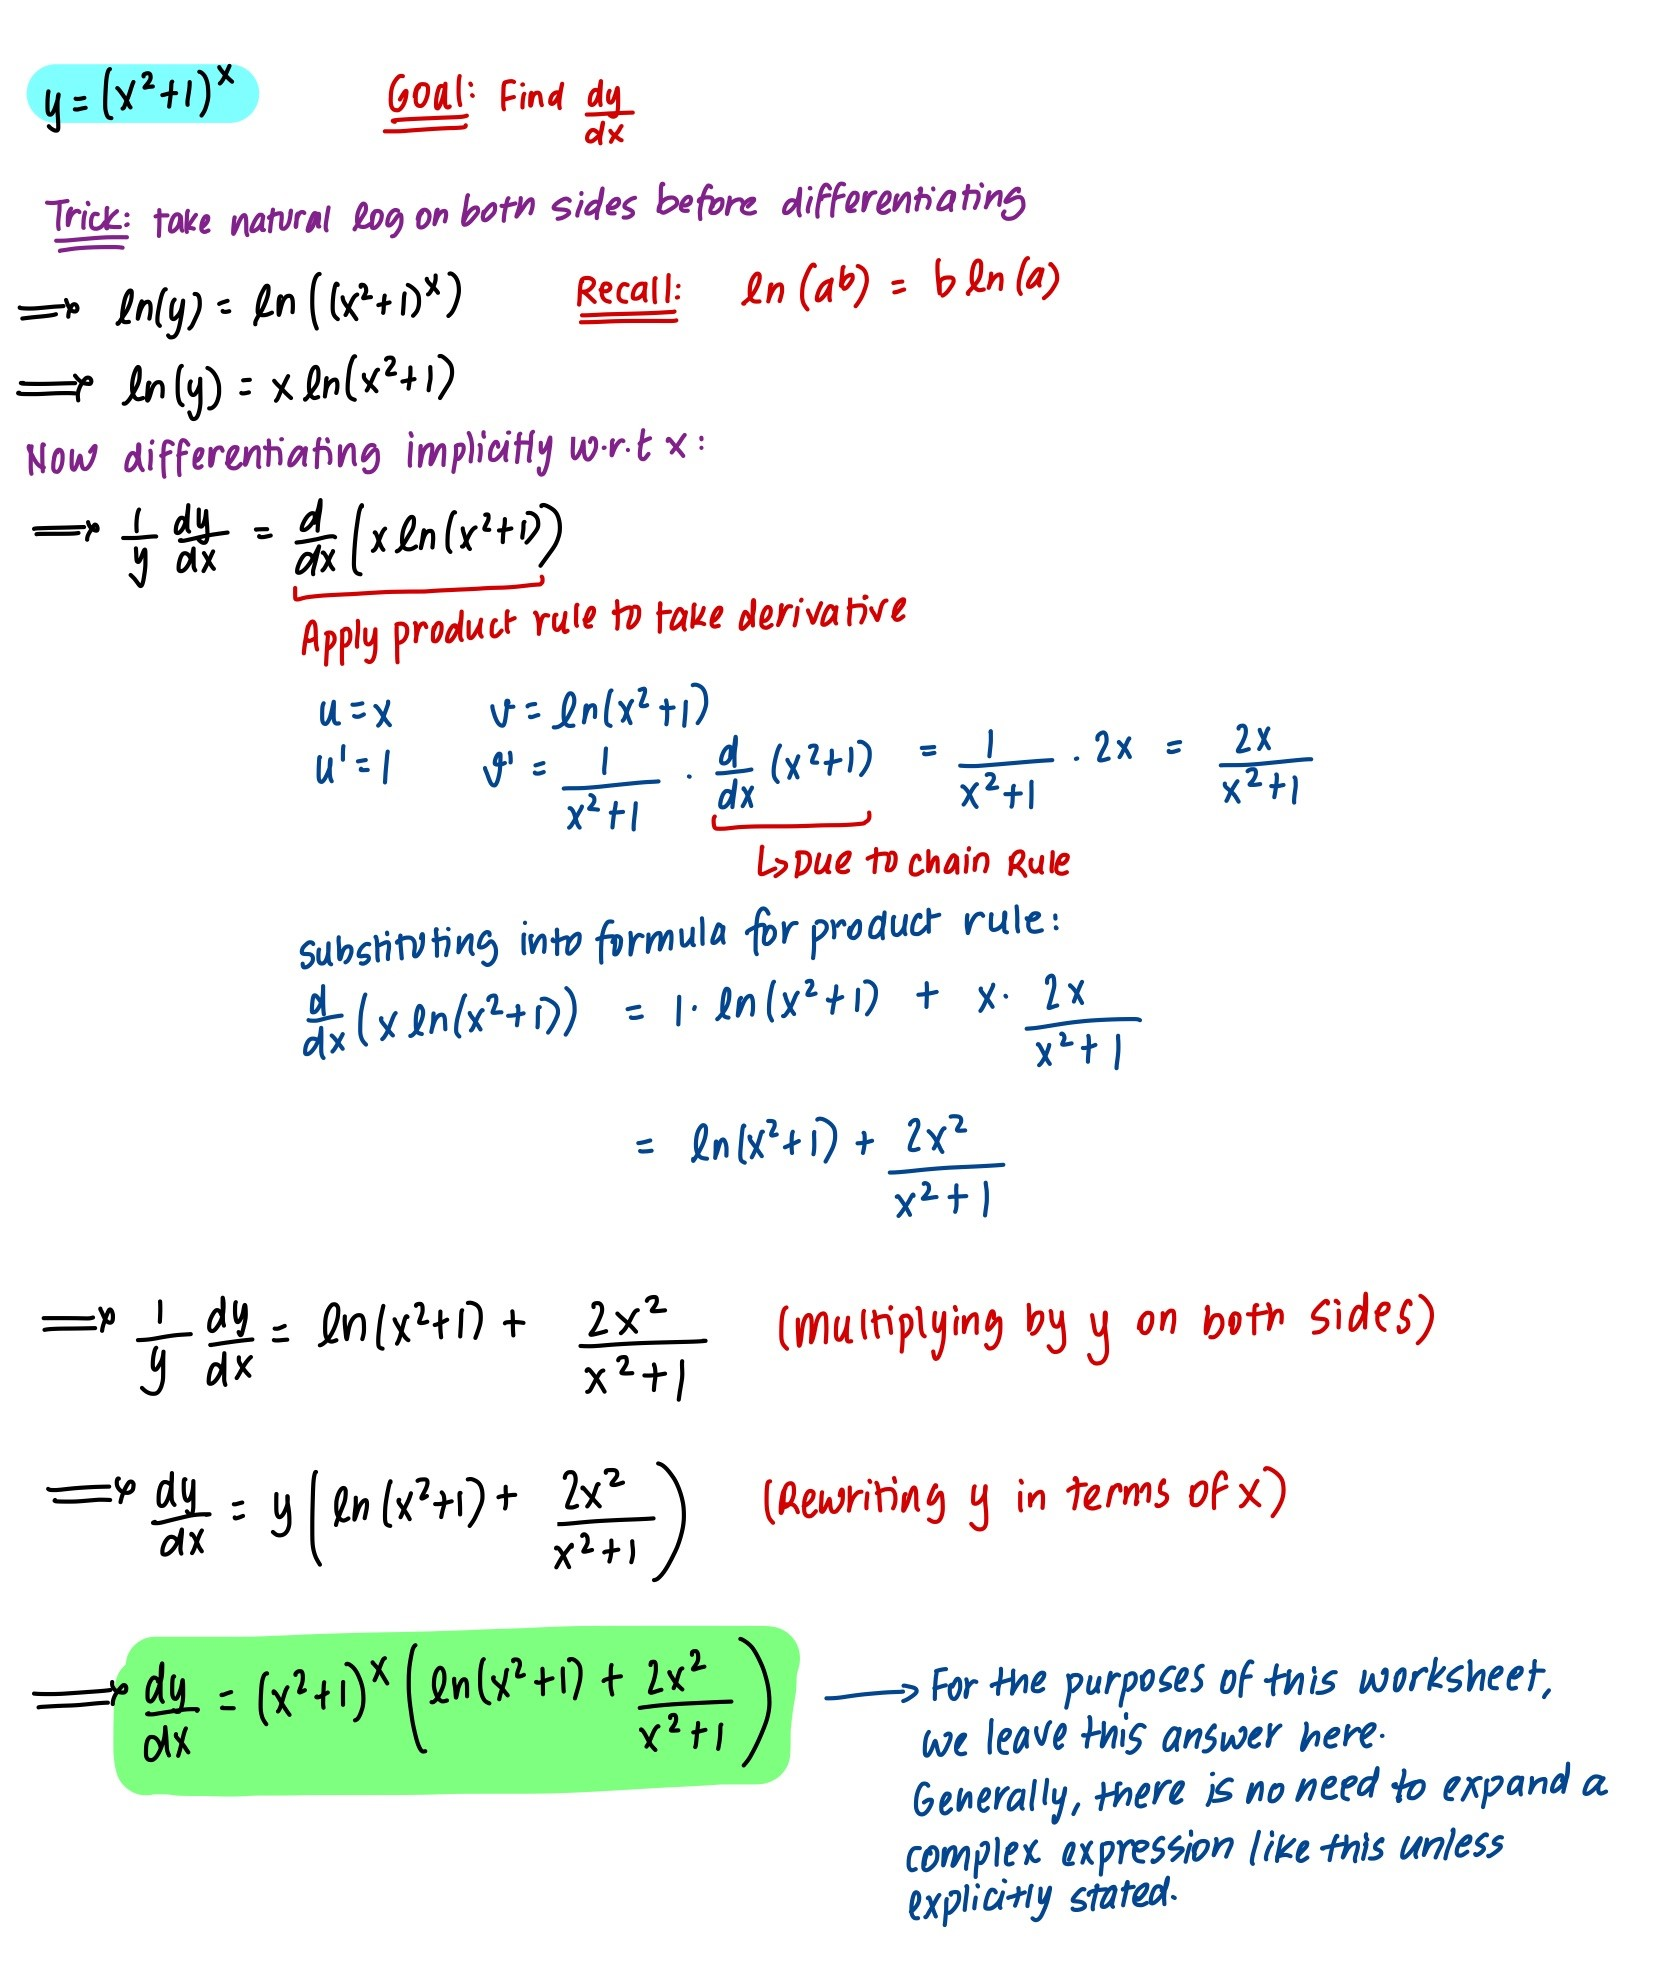
\includegraphics[width=0.9\linewidth]{Q1.3.jpg}
        \label{fig:Q1.3}
    \end{figure}
    \newpage
    \item $y = \ln(\sin(x^2))$
    \begin{figure}[H]
        \centering
        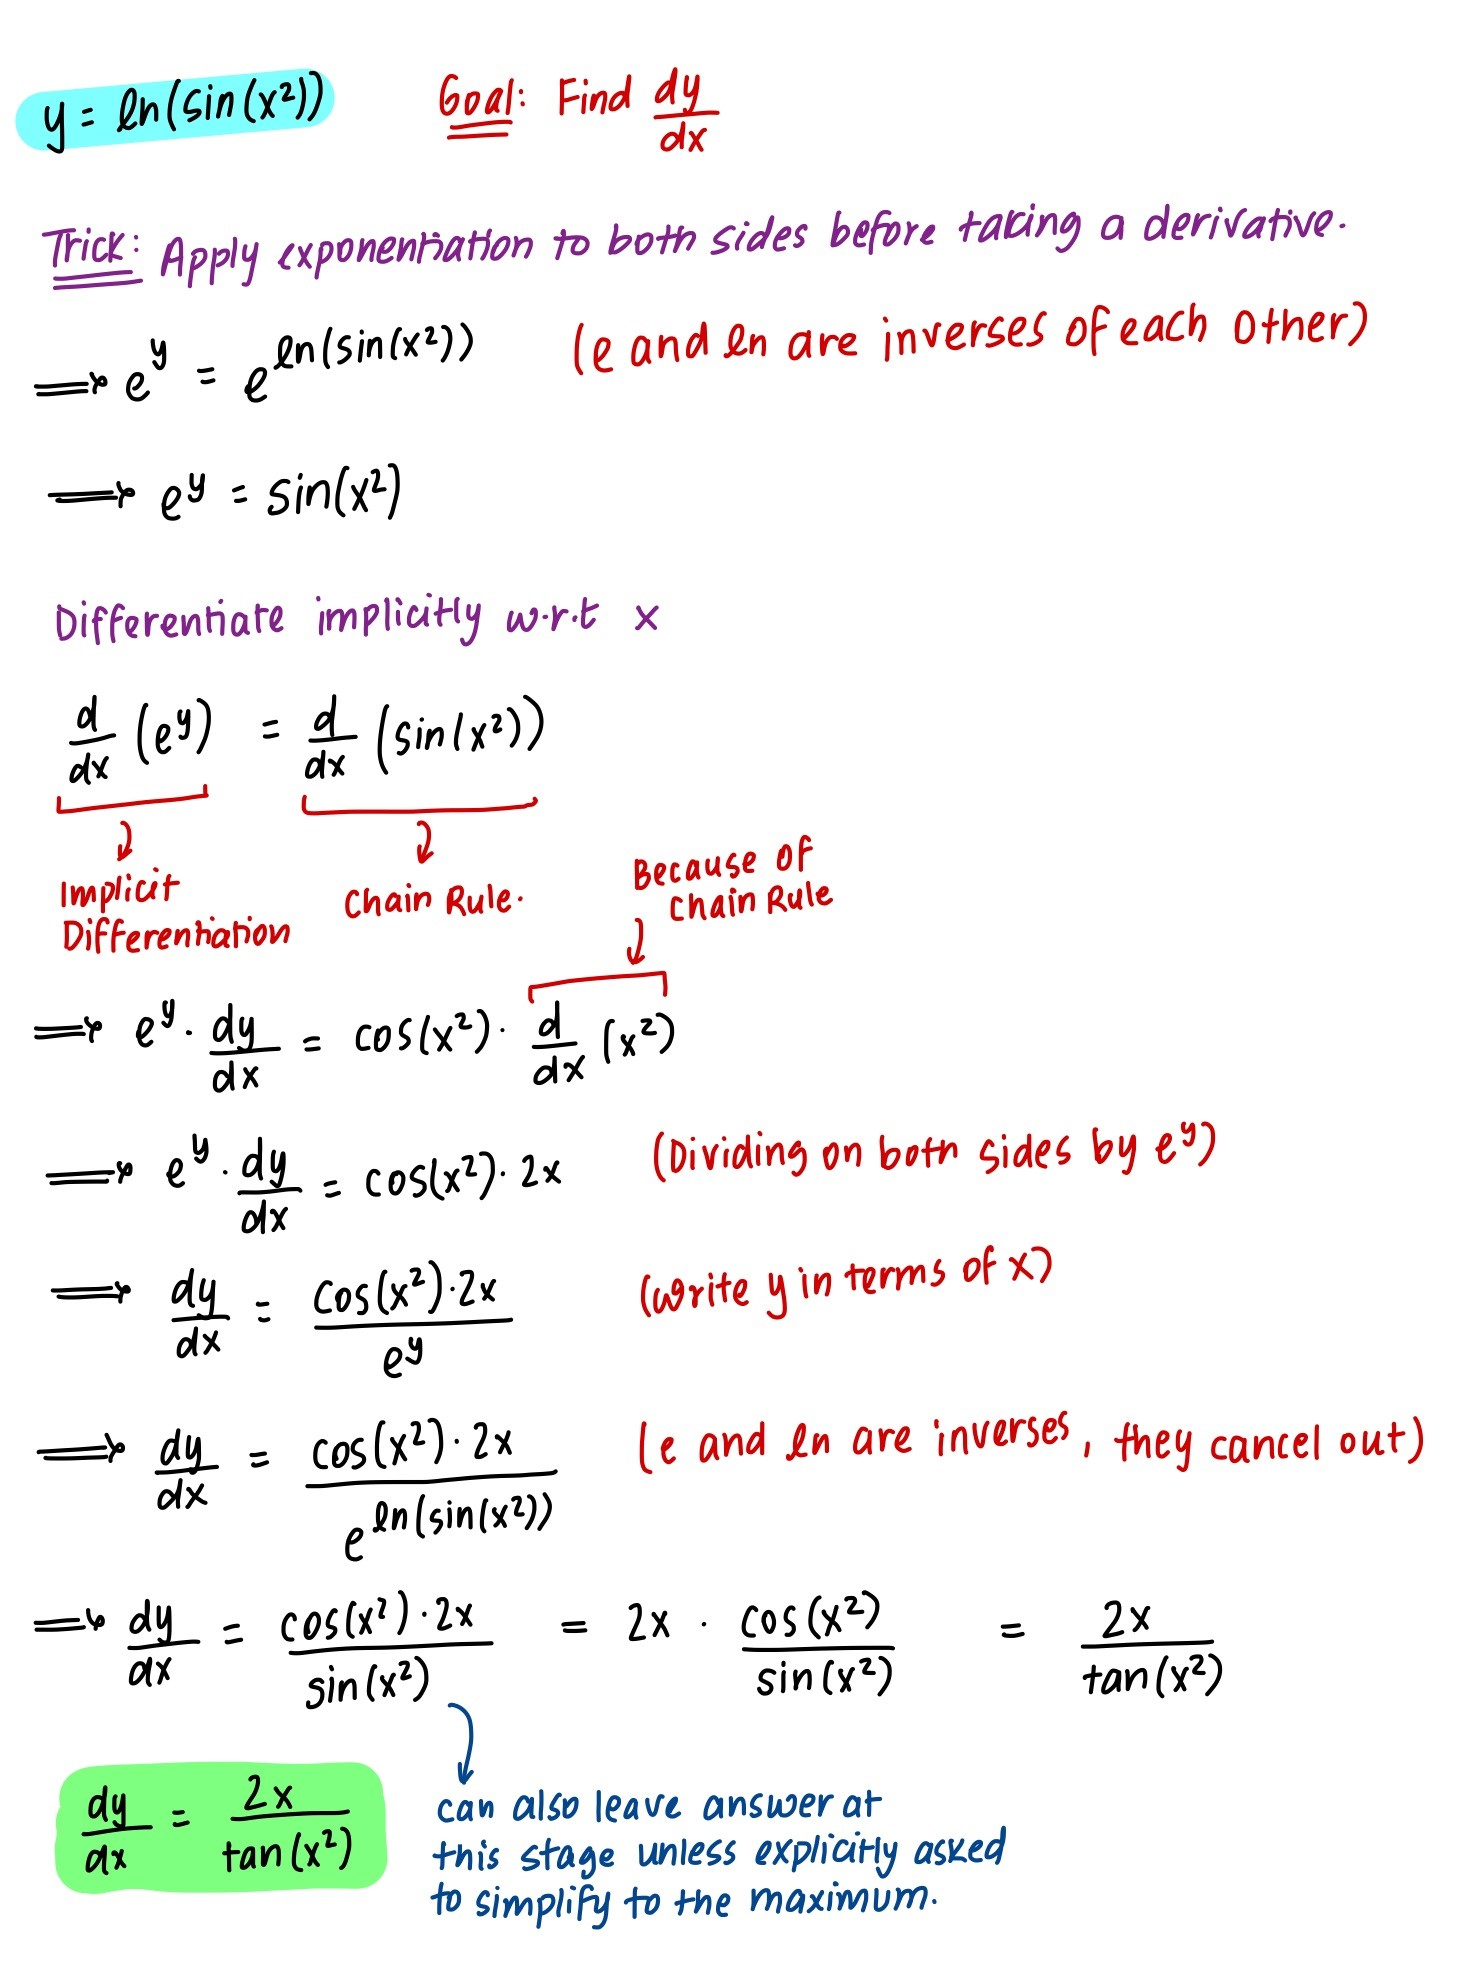
\includegraphics[width=0.9\linewidth]{Q1.4.jpg}
        \label{fig:Q1.4}
    \end{figure}

\end{enumerate}

\end{document}
